%%%% ijcai19.tex

\typeout{IJCAI-19 Instructions for Authors}

% These are the instructions for authors for IJCAI-19.

\documentclass{article}
\pdfpagewidth=8.5in
\pdfpageheight=11in
% The file ijcai19.sty is NOT the same than previous years'
\usepackage{ijcai19}

% Use the postscript times font!
\usepackage{times}
\usepackage{soul}
\usepackage{url}
\usepackage[hidelinks]{hyperref}
\usepackage[utf8]{inputenc}
\usepackage[small]{caption}
\usepackage{graphicx}
\usepackage{amsmath}
\usepackage{booktabs}
\usepackage{algorithm}
\usepackage{algorithmic}
\usepackage{epstopdf}
\urlstyle{same}

% the following package is optional:
%\usepackage{latexsym}

% Following comment is from ijcai97-submit.tex:
% The preparation of these files was supported by Schlumberger Palo Alto
% Research, AT\&T Bell Laboratories, and Morgan Kaufmann Publishers.
% Shirley Jowell, of Morgan Kaufmann Publishers, and Peter F.
% Patel-Schneider, of AT\&T Bell Laboratories collaborated on their
% preparation.

% These instructions can be modified and used in other conferences as long
% as credit to the authors and supporting agencies is retained, this notice
% is not changed, and further modification or reuse is not restricted.
% Neither Shirley Jowell nor Peter F. Patel-Schneider can be listed as
% contacts for providing assistance without their prior permission.

% To use for other conferences, change references to files and the
% conference appropriate and use other authors, contacts, publishers, and
% organizations.
% Also change the deadline and address for returning papers and the length and
% page charge instructions.
% Put where the files are available in the appropriate places.

\title{ImageNet-trained CNNs are biased towards texture; increasing shape bias improves accuracy and robustness}

% Single author syntax
\iffalse
\author{
    Sarit Kraus
    \affiliations
    Department of Computer Science, Bar-Ilan University, Israel \emails
    pcchair@ijcai19.org
}
\fi

% Multiple author syntax (remove the single-author syntax above and the \iffalse ... \fi here)
% Check the ijcai19-multiauthor.tex file for detailed instructions

\author{
Andre Diler$^1$
\and
Mehdi Chaid$^1$\and
Abderahmane Bouziane$^1$\
\affiliations
$^1$Département GIGL Polytechnique Montreal\\
\emails
andre.diler@polymtl.ca,
mehdi.chaid@polymtl.ca,
abderahmane.bouziane@polymtl.ca
}

\begin{document}

\maketitle

\begin{abstract}
The history of computer vision led us to believe that like us, Convolutional Neural Networks (CNNs) would recognize 
objects mainly by their shapes. The paper we reproduced here introduces a novel hypothesis:
modern state of the art CNNs are more biaised towards textures than shapes. 
The autors verified their theory through multiple experiments,
and were able then to train CNNs to better recognize shapes, and surpass the state of the art models on Imagenet classification.
\end{abstract}

\section{Introduction}

% https://hackernoon.com/a-brief-history-of-computer-vision-and-convolutional-neural-networks-8fe8aacc79f3

Modern Convolutional Neural Networks reach very high performances on complex computer vision tasks like
Image classification and Image Segmentation
These performances are comparable with human perception and they come from a long history of studies.
These studies led us to believe that CNNs are shape-biased. \\  
\noindent
The first proof that edges are fundamental for vision came from a very influencal study of cognition:
  “Receptive fields of single neurons in the cat’s striate cortex”
described how biological neurons extracted features from images. 
It showed that certain types of neurons were activated by edges. \\
\noindent
The convolution of an image with a sobel filter is known to extract edges.
Other filters can extract other image features. However, the filters had to be handcrafted, and
the most significant features of an image had to be determined by a human.

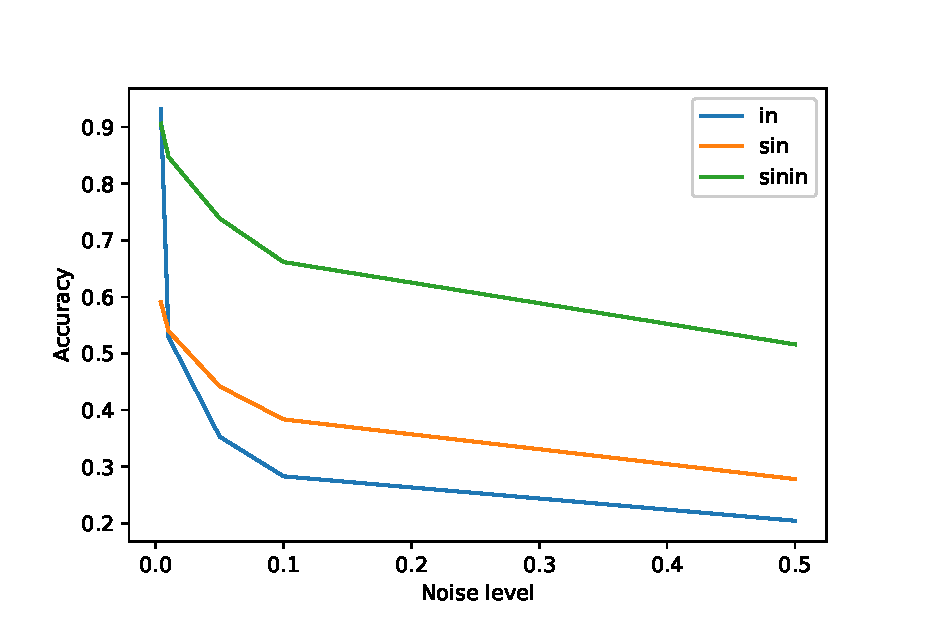
\includegraphics[width = 0.5\textwidth]{imgs/uniform}

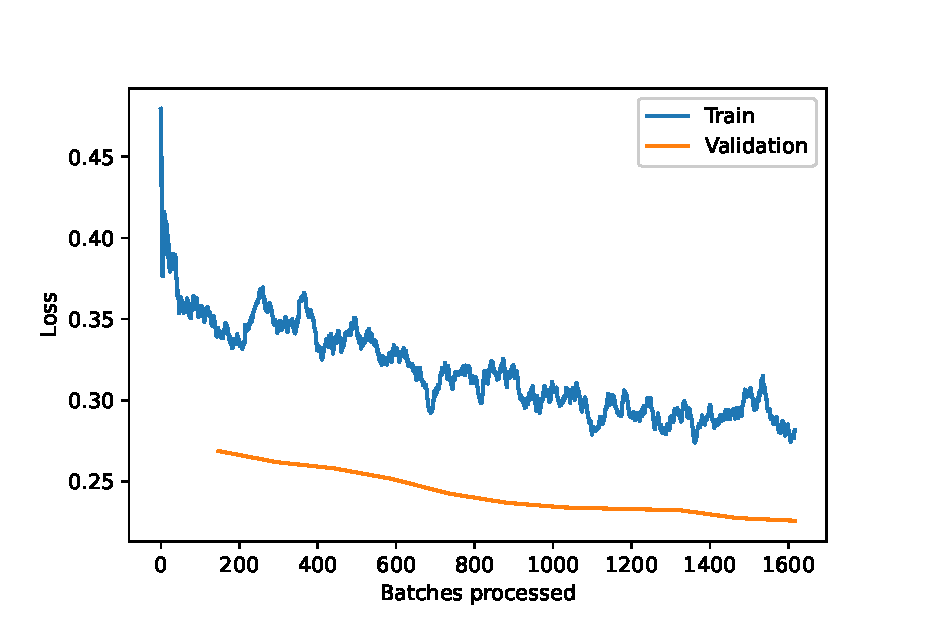
\includegraphics[width = 0.5\textwidth]{imgs/sin-in/loss}

Another paper showed that vision was hierachical. Low-level features (simple shapes like lines)
were combined to recognize high level features (like wheels, windows ...).

The famous Neocognition paper was the implementation of the idea of hierachical vision.
This multilayered neural network included convolutional layers with wheighted receptive fields (filters).
It was the first deep neural network.

The first modern convnet was LeNet \cite{Lecun98gradient-basedlearning}
It used backpropgation to automatically learn the filter values to extract meaningful features in images hierachically.
All the modern ConvNets are inspired from this network.

ConvNet were considered like a black box for a long time.
This is why efforts were made to analyze the internals of these networks.

The shape hypothesis is that "High-level units appear to learn
representations of shapes occurring in natural images” \cite{Kriegeskorte029876}
This hypothesis is widespread in the comunity, and
it is understandable given the history of computer vision.
There are a lot of experiments comparing human vision with computer vision.
X states that "implicitly learn representations of shape
 that reflect human shape perception".
Y said that "that  state-of-the-artone  shot  learning  models  trained  on  ImageNetexhibit  a  similar  bias  to  that  observed  in  hu-mans:  
they prefer to categorize objects according  to  shape  rather  than  color" \cite{ritter2017cognitive}

However, several studies raise doubts about this hypothesis.
According to X, CNNs are able to classify texturised images even if their shape structure is destraoyed.
Moreover, Y showed that CNNs with constrained receptive field sizes can reach competitive accuracies on ImageNet.
It is worth noticing that small receptive fields cannot capture the overal shape of an image.
These results have led the authors of the paper we reproduce \cite{geirhos2018imagenettrained} 
to emit a new hypothesis: the texture hypothesis where "in contrast to the
common assumption, object textures are more important than global object shapes for CNN object
recognition".

Our objective is to test these hypothesis with diverse experiments.

\section{Methodology}

\subsection{Dataset}

We used Imagenette \cite{fastai2019} a subset of ImageNet dataset created 
by fastai to do our experiments.
This ensured that our results are comparable, and that the dataset is not too large.
Imagenette contains 13394 images.
Imagenette's train/test split is 70/30: 9469 images for the train and validation set, and 3925 images for the test set.
It contains 10 easily classigied classes from Imagenet: 
(tench, English springer, cassette player, chain saw, church, French horn, garbage truck, gas pump, golf ball, parachute)
The classes are balanced with around 950 images in each one.

This dataset is more easily classifiable than Imagenet in less time, which fits our purpose.
We used the '160px' version of the images, where the shortest size of the images are resized to that size, 
with their aspect ratio maintained.


\subsection{Style Transfer}

We applied style transfer on Imagenette to replace the original texture using the code originally used in
the paper with a random texture. 
Style transfer consists in XXX
We used AdaIN to 
We used the implementation made by XX \cite{stylizeddatasets2019}
This procedure ensures that the images conserve their edges, but not their textures.
We used samples from the Describable Texture Dataset \cite{cimpoi14describing}.



\subsection{ResNet}

TODO


\subsection{Cue Conflict ???}

TODO MAYBE ?

\newpage
\section{Experiments}

The authors of the original paper trained multiple models, 
namely Resnet-50, BagNet-33, BagNet-17 and BagNet-9

MODELS
TEXTURES
DATASETS

\subsection{Texture biais hypothesis}
% The first experiment of this analysis was to reproduce the original experiment of the paper with imagenette-160 
% and handpicked images and textures. 
% We then trained a ResNet-18 to classify the chosen images and visualize the results.
% Figure 1 below shows the result of classification for a content image (a), texture image (b) and stylized image (c).

The first experiment conducted by the authors was to visualize the texture biais 
through image classification on a stylized image. 
Their hypothesis was that the textured image would be classified as the texture representation, rather than 
the underlying content using the shapes, which is contrary to popular belief. \\
\noindent
We've reproduced their experiment in figure 1, % TODO: ADD LINK ??
using the picture of an English Springer as our content image (a), 
a colorful parachute as our texture image (b),
and a stylized version of the Springer (c) using AdaIN style transfer 
(Huang \& Belongie, 2017) % TODO: ADD REFERENCE TO STYLE TRANSFER
to introduce a texture-shape cue conflicts.

\begin{figure}[h!]\center
  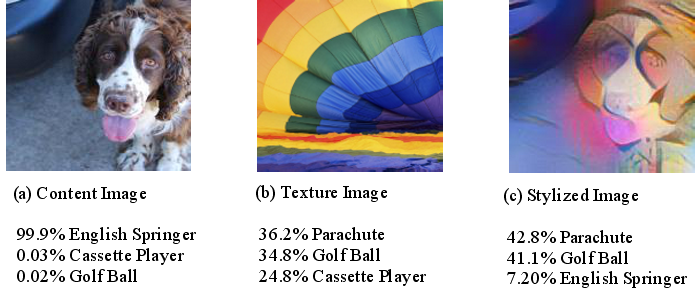
\includegraphics[width=0.47\textwidth]{imgs/results-textures}
\end{figure}

\noindent
As we can see, we've obtained the same classification results as the authors, 
where the stylized image was being recognized as the parachute texture
rather than the underlying Springer content.

\subsection{Stylized-imagenette-160}

In order to reduce the texture biais of ResNet-18, and introduce a more familiar shape biais, 
the authors trained their model on a stylized version of Imagenet. 
Due to time and material constraints, we've decided to use 

\subsection{Overcoming the texture biais}

EXPERIENCE IN SIN ETC

\subsection{Shape-ResNet}

JOINTLY ON SIN IN AND FINETUNE

\subsection{Noise resistance}

EXPERIENCE ABOUDELOU

\newpage
\section{Approach analysis}

Idk what tf goes here

\newpage
\section{Conclusion}

This is where we conclude bois

% To begin with, we reproduced the first experiment of the paper. This experiment
% is represents the misconception we have about how CNNs learn.

% Figure Mehdi

% We can see that the pretrained CNN recognized the elephant with just its texture.
% More interestingly, it recognized it classified the cat shape with elephant texture as an elephant.
% The texture hypothesis is more likely to be true.
% Let's define more robust experiments to verify that.

% \newpage
% \subsection{Texture bias of CNNs}

% General explanation

% \subsubsection{IN to IN}
% expected results
% \subsubsection{SIN to IN}
% expected results

% \subsection{Dataset}

% Details on dataset creation

% \subsection{Resistance to noise}

% Experiences Abder
% Data generation

% \subsection{Training}

% Details of ResNet model
% Hyperparams
% Nb Epochs
% FineTuning method

% \section{Results}

% \subsection{Texture bias of CNNs}

% \subsection{Resistance to noise}


% \section{Discussion}

% \subsection{Texture bias of CNNs}

% \subsection{Resistance to noise}


\newpage
\appendix

%% The file named.bst is a bibliography style file for BibTeX 0.99c
\bibliographystyle{named}
\bibliography{ijcai19}

\end{document}

